%We document the retrieval, enhancement, labelling and augmentation of [the|our] data set [used for the experiments].
% We document how we retrieve, enhance, label and augment our data set.
We document the retrieval, enhancement, labelling and augmentation of our data set.

	\subsection{Database}
We have decided to use digital over film mammograms. Digital mammograms are sharper and do not have marks, stamps or other artifacts present in digitised film mammograms. On the downside, because the technology is newer it may be harder to obtain big databases and given its higher resolution they are normally heavier in terms of disk space. We believe the network will be able to pick up better features from the higher quality images and that the size on disk will not be a trouble given the storage availability on current computers. A small number of examples in the database is a big problem and some alternatives are offered below in case the network is not able to learn with the available data. For these reasons, we have decided to use initially the BCDR-DM and INbreast databases.
%BCDR
%A small desciption is offered below.

%	\subsubsection{BCDR-DM}
%	Yet to write
% Files and how are they organized. Data available per case and per mammogram. How are boundaries written. formats, etc.
% 159 calcifications, 36 micro, 11 micro+calcif, thus 108 micro or calcif. 106 nodule, 20 nodule+ calcific, 11 nodule + micro
	
	\subsection{Image retrieval/Preprocessing}
	We document here the decisions taken to obtain the small image patches $x$ and its respective labels $y$ from the chosen databases.

\paragraph{Image dimensions}
We use square image patches because they are common in practice and simplify data augmentation. To define the size we have to consider two aspects: keeping a manageable input size for the network (in pixels) and capturing the entire lesion in the image patch (in mm).

The smallest microcalcification worth considering could be as small as 0.16 mm~\cite{Lo1998}, thus the spatial resolution should be at most 0.16 mm. The standard definition of a cluster of microcalcifications is of 5 or more inside a 1 $cm^2$ area~\cite{Sickles2013}, thus the entire image patch should cover at least a 1 $cm^2$ area. Using an image patch of $64  \times 64$ pixels we cover an image area of 1 $cm^2$ with a pixel size of 0.156 mm. 
% Pizel size .16 , i get 1.024 cm size.
Mass sizes (length of the long axis) vary from 5 mm to 20 mm~\cite{Sahiner1996}~\footnote{Bigger masses are easily detectable by touch and thus less important for our purposes.} There is not really any restriction on spatial resolution other than it being good enough to capture texture information. Again, using an image size of $64 \times 64$ pixels we can cover a 4 $cm^2$ area (2 cm per side) with a spatial resolution of 0.313 mm.
% pixel size 0.39 equals area 25 mm
% pixel size .4 mm equals ara 25.6 mm (exactly the size in Sahiner1996)

The low spatial resolution (big pixel sizes), however, reduces the quality of the input images. An alternative could be to use $127 \times 127$ image patches with 0.079 mm and 0.157 mm pixel sizes for microcalcifications and masses, respectively, aplying a bigger filter on the first convolutional layer, for instance, a $5 \times 5$ filter with stride 2 and padding 2. This allows us to have bigger input images with a negligible increase in the number of parameters. Whether the results improve or not is not clear at this point.

Although we use the same input size (either $64 \times 64$ or $127 \times 127$) for microcalcifications and masses they do not cover the same area in the mammogram. We need to use two different sizes because if we preserve the spatial resolution of microcalcifications, the 1 $cm^2$ area would not be able to contain the entire mass meanwhile if we use a resolution closer to the one used for masses, small microcalcifications will dissapear and the 4 $cm^2$ area would have way too much noise compared to the size of the cluster of microcalcifications.
%An alternative is to use a $128 \times 128$ pixels image patch with 0.16 mm, this will result on the same 4 $cm^2$ area needed for masses with the spatial resolution needed for microcalcifications allowing us to train a single network for both kinds of lesions. Nonetheless, this has some critical flaws: the number of learnable parameters will almost double, the GPU may run into memory bottlenecks because of the increased number of parameters and unnnecesary details (noise) will be included in the image.

\paragraph{Cropping}
To obtain the image patches from the entire mammogram we slide a square window across the mammogram similar to the way a convolutional filter moves accross an image and store the image patch directly beneath it. This generates a big number of small patches from each mammogram and takes advantage of the translational invariance of our data, i.e., a breast mass will continue to be a breast mass no matter its position in the image patch.

An alternative is to sample the desired number of image patches at random positions from the mammograms.

\paragraph{Stride}
We chose a stride of 1 mm for the microcalcifications case and 2 mm for breast masses. This is midway between a very small stride, say 0.05 mm, which produces many image patches with maximum overlapping and big strides, say 1 cm, which produces fewer patches with little to no overlapping. We use a rather small stride to have a lesion appear in various image patches (although in a slightly different place in each one) and to produce a good number of patches from the original image. We use no padding.

When sliding the window starting from the upper left corner of the original image it is possible that due to a dimension mismatch pixels in the rightmost and bottom strips do not appear in any image patch, this is not a problem given that the lost strips are very thin ($<$ 1 mm for microcalcifications or  $<$ 2 mm for masses) and they are normally part of the background.

\paragraph{Background}
Mammograms capture images of the breast against a black background which covers a good part of the mammogram. We delete any image patch which is 25\% or more black. No important information is lost in this process because the same part of the breast which appears in a deleted patch also appears on other image patches with less black background. A remaining question is how will the trained convolutional network react when presented with an all black input, for example, when slided across the background of a test mammogram. In practice, however, this is not relevant because it is clear that no lesion could occur outside the breast. 

An alternative is to preserve all images and let the network learn that black images are negative examples but this seems rather wasteful.

\paragraph{Assigning labels}
Once each image patch is obtained we need to assign labels to it. All image patches are initially labelled as negative (or no lesion) and only those where a lesion is present are labelled as positive. There are many ways to define the presence of a lesion in an image: (1) if a percentage of the lesion, say 70\% or more, appears in the image, (2) if a percentage of the image is covered by the lesion and (3) if a part of the lesion appears in the middle of the image.

We have chosen the last option to define the presence of a lesion because of three reasons: it is simple to implement, it somehow includes the other methods given that when a lesion appears on the middle of the image patch the rest of it will probably also appear on that patch and finally it encourages the convolutional network to output true only when the lesion appears in the center of the patch but not anywhere else which may give us more granular results when using it on the entire mammogram. The downside is that when a lesion is found on the outside of the image patch (in a corner, for example) it will be labelled as a negative example in the training set and may difficult the learning because even though the lesion is there we are training the network to answer negatively; if this effect actually occurs is not clear. \cite{Ciresan2013} uses this method to label its image patches.

Using the first or second option is a viable alternative although they come with their own caveats, for instance, it could be hard to calculate the area of irregular objects or the lesion could be so big that even covering the the entire image patch area it would still not account for 70\%.

\paragraph{Label information}
We will use the type of lession (mass, clustered microcalcifications or normal) and the malignancy (bening, malignant or nothing) to train our networks.
% For the detection case, we do not consider malignancy it is lesion vs normal, for diagnosis we only consider the malignant ones.
% LeCun says convnets like to have many categories because they can identify better features early in the processing. Maybe it is better to have the same convnet for different lessions.

Databases normally offer adittional information such as age of the patient, breast density, family clinical history, assesment of the subtlety and malignancy of the lesion, etc. This information could be used as complementary features before classification or as labels for the network. In this stage we use only the mammograms with the labels stated above (binary classification).


\paragraph{Image enhancement}
In theory we want to perform classification on the raw images (without any preprocessing) so we store the raw image patches and their labels as the base training set and perform any image enhancements during training whenever possible. There is a set of simple contrast adjustments that could be applied: normalization assigns 0 to the minimum gray value in the image and 255 (or the maximum available value) to the maximum gray value in the image and stretches the rest of the values linearly, background reduction plus normalization is similar except that all values below a given threshold (the mean of all pixel values in the image) are mapped to zero and the rest is normalized effectively reducing all small variations in the background to black and histogram equalization which tries to distribute the gray values evenly on the histogram of the image. An example of each method is shown in Fig.~\ref{fig:PreprocessingTechniques}.
\begin{figure}[h!]
	\centering
	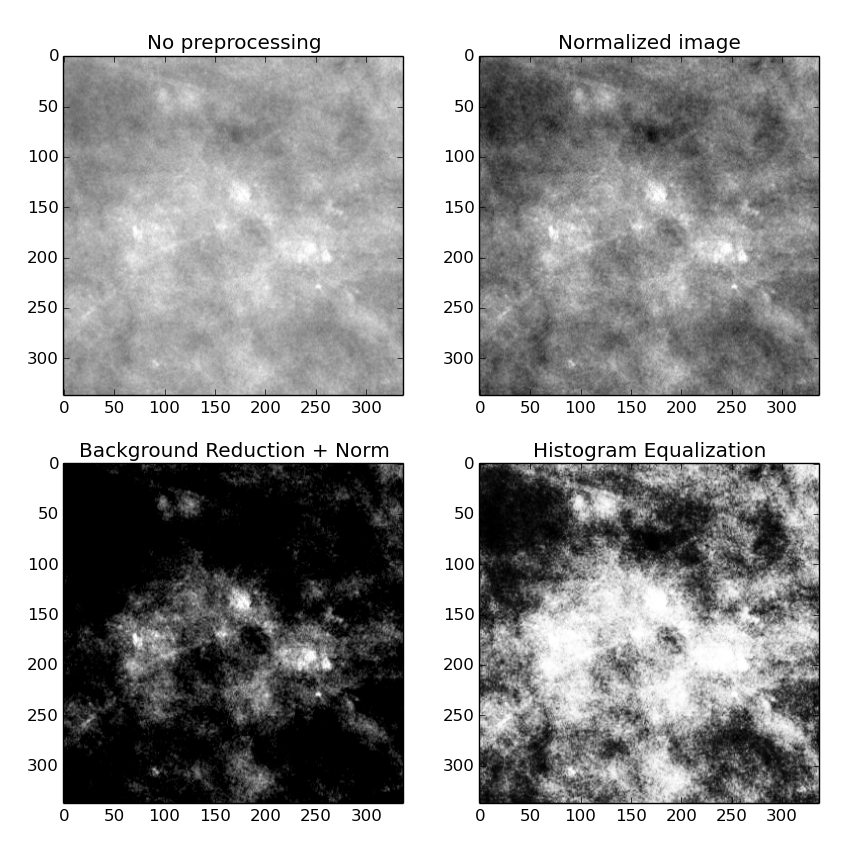
\includegraphics [width = 0.7\textwidth]{plots/mcDiffPreprocessings.png}
	\caption[Example of constrast adjustment techniques]{Example of simple contrast adjustment techniques applied to an image with a cluster of microcalcifications. Normalization takes the range of gray values and stretchs it up to linearly cover the entire range available. Background reduction assigns 0 to every pixel below the mean of the pixel values and applies normalization. Histogram equalization distributes the gray values more evenly in the histogram of the picture.}
	\label{fig:PreprocessingTechniques}
\end{figure}

We use background reduction plus normalization because it increases the signal to noise ratio, i.e., highlights lesions over normal breast tissue. On the downside, it also highlights dense structures (which could increase false positives) and may destroy important texture information by blending it with the background; using normalization only could produce better results. Unpreprocessed images seem too noisy and histogram equalization is too destructive for our purposes.

\paragraph{Data augmentation}
We augment each enhanced image by using 4 rotations (at 0°, 90°, 180° and 270°) of both the original image and a horizontally flipped version of it, thus we increase our data set by a factor of 8. Both rotations and reflections preserve the original label. In principle it is not neccesary to store the augmented images because they can be easily generated during training but if the disk space is not prohibitive explicitly storing them simplifies training.
%Does it affect to present all different augmentations of the same image in one batch rather than in different batches?

%TODO: Is feature normalization needed? It does put everything on -1 to 1 range (instead of 0-256, 0-2048, etc.). if it doesn't affect the results better do it

\paragraph{Resizing}
We have to resize the images to achieve the desired patch size. There is a couple of decisions to take in this part: the type of interpolation to use and whether image enhancement should be performed before or after resizing. After some experiments neither decisions proved to be very important for the resulting image patches. We choose the Lanczos interpolation recommended for downsizing in the PILLOW Python Image Library. Enhancements are executed on each particular patch before being scaled to their final size. Figure~\ref{fig:ResizingInterps} shows the effect of using the Bicubic or Lanczos interpolation scheme for resizing both before and after enhancement. Results are similar under all configurations.

\begin{figure}
	\centering
	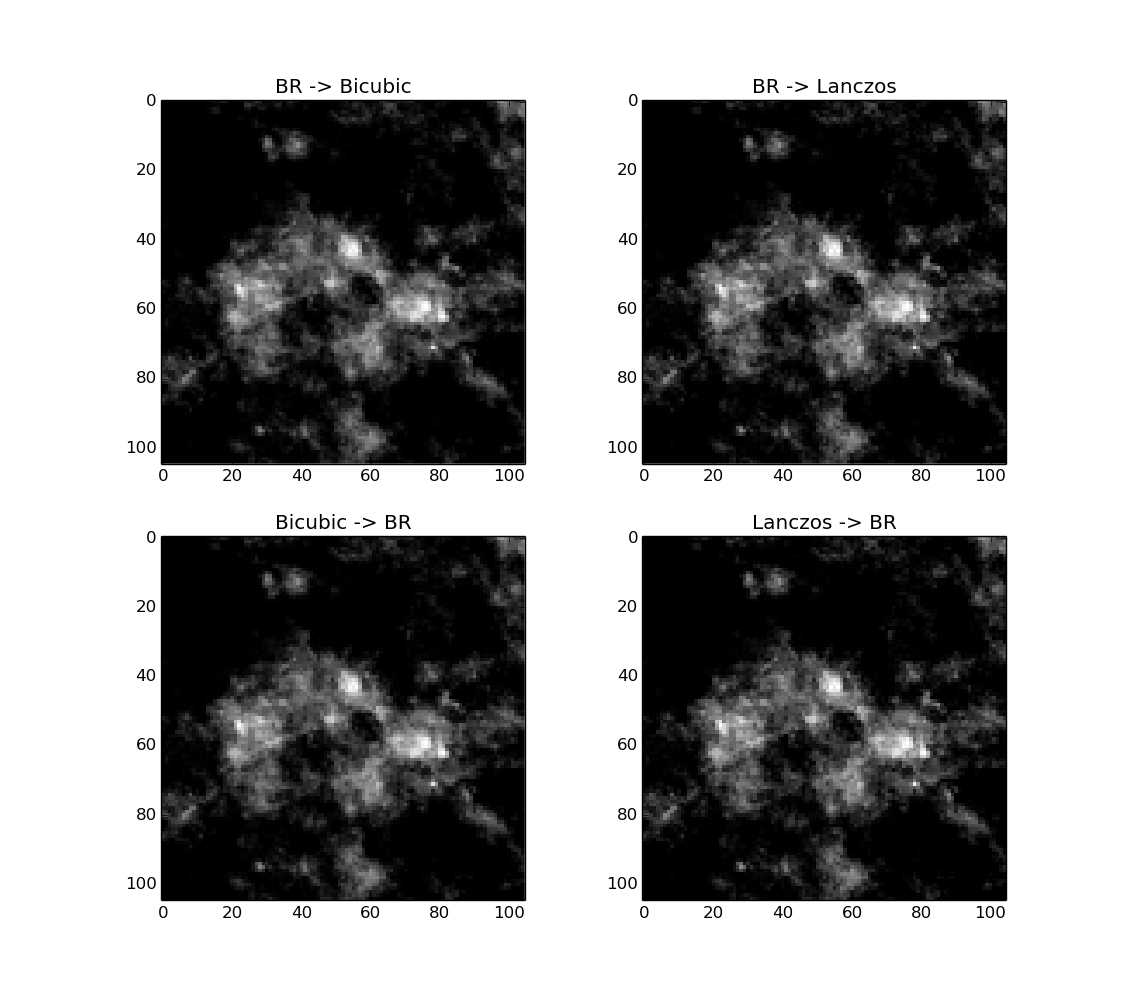
\includegraphics [width = 0.8\textwidth]{plots/mcDiffResizings.png}
	\caption[Example of resizing schemes]{Example of different resizing schemes applied to an image with a cluster of microcalcifications. Bicubic and Lanczos inteprolation is used for resizing an original 317 pixel image to 105 pixels before and after enhancement (background reduction plus normalization) as shown by the arrows in the subtitles. Results are virtually undistinguishable.}
	\label{fig:ResizingInterps}
\end{figure}

\paragraph{Storage}
For each mammogram we will generate a single 3-dimensional matrix ($64 \times 64 \times x$)  containing all $x$ preprocessed patches obtained from the mammogram. This matrix will be stored as a .pch file with the same name and on the same directory as the original image.
 
% Images will not be zero-centered , normalized or whitened. global contrast
% with global contrast stretching will make comparisons across patients not good, because if a pixel is very bright in one patient that is only important with respect to that patient and it may end up (by contrast stretching) having the same value that the pixel in another mammogram who wasn't as bright but was the brightest of the mammogram. i think this makes sense because masss are going ot be bright but only in relation to the patient, maybe one has very fatty tissue so all is white and others have very clear tissue.
% Labels are background, lession and breast tissue. 
% Or could I crop the figure closely to the background and then calculate over all spaces (nop). How do you backpropagate through this mask? Just assign perfect scores to evry position in your predictions that is background (check where is the background in the mask), that way it will be counted by normal gradient, but it will not contribute. I could add a layer at the end (or before the loss function), that sets the gradient to zero in the backwards pass if the position it is viewing is  a background pixel. that'll do it.
% Or i could assume that anythong under the global mean won't be a mass and then during classification and during training just set them to black/treat them as background (this owuld be the equivalent ot train them and test them only on those pixels that are greater than the global means0). But maybe this then reduces the data se too much and I won't learn. More or less half the values are gonna go to zero. I would need to create a label where evrything below the global mena is background (0), any lession is (1) and any other breats tissue  is (0.5). Overcomplicated, better let the network also see some black patches maybe that help it. do get rid of backgorund, though.
% Or look for clusters/connected components of values in the mammogram (after background reduction) and crop those (boundig box) and train on them, this way i don't need to send the big mammogram but just these cropped parts (in case there is not enough memory). Note: for components to be separated they have to be at least 128 pixels apart (because i have to preserve surroundig region, too). This is not gonna work, because the connected component is going to be the entire breast area, see some examples if you doubt it.
% Or maybe just crop after background reduction to get rid of some parts that are not needed. Will I win a lot, though?. It looks like I won't. Don't do
	
	\subsection{Data augmentation}
	Rotations and flipping of original big images. the breast and cannals, and nipple may be very different at 90 and 270, flipping an 180 seem fine. Or maybe not.


	\subsection{Data division}
	70/15/15 is a good split. stratified per patient, this total number of patients in each set and this total number of mammograms (after augmentation) and this total number of lesions.
% do alittle table with rows being percentage of data set, patients, mammograms, # of masses and columns being training, validation test.That way I syummarize all information. i can also add a total column, summing over all trainng and test set.
